 	\documentclass{article}

%Header Dimensions
%https://tex.stackexchange.com/questions/40183/problem-with-the-header-footer-width#40184
\usepackage[margin=0.5in,bottom=0.5in,top=0.5in]{geometry}

%Package required for empty set
\usepackage{amssymb}

%Package required for Comb/Perm symbol and matrices
\usepackage{amsmath}

%Package for graphics
\usepackage{graphicx}

\begin{document}

	
%%%%%%%%%%%%%%%%%
%CUSTOM COMMANDS%
%%%%%%%%%%%%%%%%%

	%This line surpresses the page number
%https://tex.stackexchange.com/questions/7355/how-to-suppress-page-number
\thispagestyle{empty}

%Make empty set pretty
% https://tex.stackexchange.com/questions/22798/nice-looking-empty-setup
\let\oldemptyset\emptyset
\let\emptyset\varnothing


%Combinatorial notation
%From https://tex.stackexchange.com/questions/107125/is-there-a-command-to-write-the-form-of-a-combination-or-permutation
\newcommand*{\Perm}[2]{{}^{#1}\!P_{#2}}
\newcommand*{\Comb}[2]{{}^{#1}C_{#2}}


	
\textbf{	Matt Fletcher MA385 Homework 1}
\smallskip

\noindent\rule{8cm}{0.4pt}

1. 

a) List all items in the sample space $\Omega$:

\{1, 0\}, \{1, 1\}, \{1, 2\}, \{1, 3\}, \{1, 4\}, \{1, 5\}, \{1, 6\}, \{2, 0\}, \{2, 1\}, \{2, 2\}, \{2, 3\}, \{2, 4\}, \{2, 5\}, \{2, 6\}, \{3, 0\}, \{3, 1\}, \{3, 2\}, \{3, 3\}, \{3, 4\}, \{3, 5\}, \{3, 6\}, \{4, 0\}, \{4, 1\}, \{4, 2\}, \{4, 3\}, \{4, 4\}, \{4, 5\}, \{4, 6\}, \{5, 0\}, \{5, 1\}, \{5, 2\}, \{5, 3\}, \{5, 4\}, \{5, 5\}, \{5, 6\}, \{6, 0\}, \{6, 1\}, \{6, 2\}, \{6, 3\}, \{6, 4\}, \{6, 5\}, \{6, 6\},

b)  List outcomes where:


A) At least 1 four is rolled: \{1, 4\}, \{2, 4\}, \{3, 4\}, \{4, 0\}, \{4, 1\}, \{4, 2\}, \{4, 3\}, \{4, 4\}, \{4, 5\}, \{4, 6\}, \{5, 4\}, \{6, 4\}

B) Both Dice are even:  \{2, 0\}, \{2, 4\}, \{4, 0\}, \{4, 4\}, \{6, 0\}, \{6, 4\}

C) $A \cap B$: \{2, 4\}, \{4, 0\}, \{4, 4\}, \{6, 4\}

D) $A \cup B$: \{1, 4\}, \{2, 0\}, \{2, 4\}, \{3, 4\}, \{4, 0\}, \{4, 1\}, \{4, 2\}, \{4, 3\}, \{4, 4\}, \{4, 5\}, \{4, 6\}, \{5, 4\}, \{6, 0\}, \{6, 4\}

E)  \{1, 0\}, \{1, 1\}, \{1, 2\}, \{1, 3\}, \{1, 5\}, \{1, 6\}, \{2, 1\}, \{2, 2\}, \{2, 3\}, \{2, 5\}, \{2, 6\}, \{3, 0\}, \{3, 1\}, \{3, 2\}, \{3, 3\}, \{3, 5\}, \{3, 6\}, \{5, 0\}, \{5, 1\}, \{5, 2\}, \{5, 3\}, \{5, 5\}, \{5, 6\}, \{6, 1\}, \{6, 2\}, \{6, 3\}, \{6, 5\}, \{6, 6\}

\noindent\rule{8cm}{0.4pt}

2. 

The probability that a pet comes from a house with 3 pets:

Total number of possible pets to pick: 50. 

Number of pets that could come from a house with 3 pets: Because 7 houses each have 3 pets, there are 21 pets that could come from a house with 3 pets. 

The probability, then, is $\boxed{{\frac{21}{50}}}$. %TODO BOX

\noindent\rule{8cm}{0.4pt}

3. 

a) $P(A)$: there are 3 desired outcomes (drawing a 2,4, or 6) and 8 possible outcomes. Therefore, the probability $P(A)= \frac{3}{8}$. 

b) $P(A)'$: The complement of $A$ is the opposite. There are $5$ balls in the desired outcome; therefore, the  probability $P(A)'= \boxed{\frac{5}{8}}$. 

c) $P(A\cup B)$: The union of $\{3,4,5,6,7\}$ and $\{2,4,6\}$ is $\{2,3,4,5,6,7\}$. There are 6 outcomes in the desired set, and 8 in the total possibilities, making the probability $P(A\cup B)= \boxed{\frac{3}{4}}$. 

d) $P(A \cap B)$: The intersect of $\{3,4,5,6,7\}$ and $\{2,4,6\}$ is $\{4,6\}$. There are 2 outcomes in the desired set, and 8 in the total possibilities, making the probability $P(A\cap B)= \boxed{\frac{1}{4}}$. 

\noindent\rule{8cm}{0.4pt}

4. The probability of a blackjack from a random deck: 

There are 4 Aces in the deck. If one card is an Ace, the other card must be in $\{10, J, Q, K\}$. There are 16 cards in that set. Therefore, there are $4 * 16 = 64$ cases of a blackjack. 

There are $\Comb{52}{2}=\frac{52!}{2!(52-2)!} =52 \times 51 / 2  = 1326$ possible 2 card hands. 

$\frac{64}{1326} = \boxed{\frac{32	}{663}}$. 

\noindent\rule{8cm}{0.4pt}


5. 

There is exactly 1 case where both of the 2 contractors are selected. 

There are $7 \times 6 = 42$ possible ways to select 2 council members. 

The probability both contractors are selected is $\frac{2}{42} = \boxed{\frac{1}{21}}$. 

\noindent\rule{8cm}{0.4pt}

6. 

Simplify. See attached page for graphics. 

a) $(E\cup F) \cap (E \cup F^{C})$

I'll first work on the insides of the parentheses. $E\cup F$ is the union of $E$ and $F$, so everything that is inside both $E$ and $F$.
 

$E\cup F^C$ is $E$ unioned with everything not in $F$. So, this is everything that is in $E$ that is also not in $F$. 


The intersection  of these two sets is everything contained in both sets.  Because one set is everything in both $E$ and $F$, and the other set is everything in $E$ and NOT in $F$, this simplifies to the null set: 

$\boxed{\{\emptyset\}}$

b) $(E\cap F) \cap (E \cap G)^{C}$

Again, I will evaluate the inside of the parentheses first. 

$E\cap F$ is everything that is contained in both $E$ and $F$. This is everything inside of both the $E$ circle and the $F$ circle. 
 
$E\cap G$ is everything that is contained in both $E$ and $G$. The compliment of this is everything that is not in $E$ and also not in $G$. In a Venn diagram, this is everything outside the circles representing $E$ and $G$ but inside the universal set $U$. 

The intersect of these 2 sets is everything contained in both sets. This means that the simplification is $\boxed{\{E \cap F \cap G^C\} }$



See picture. 
\begin{figure}
	\centering
	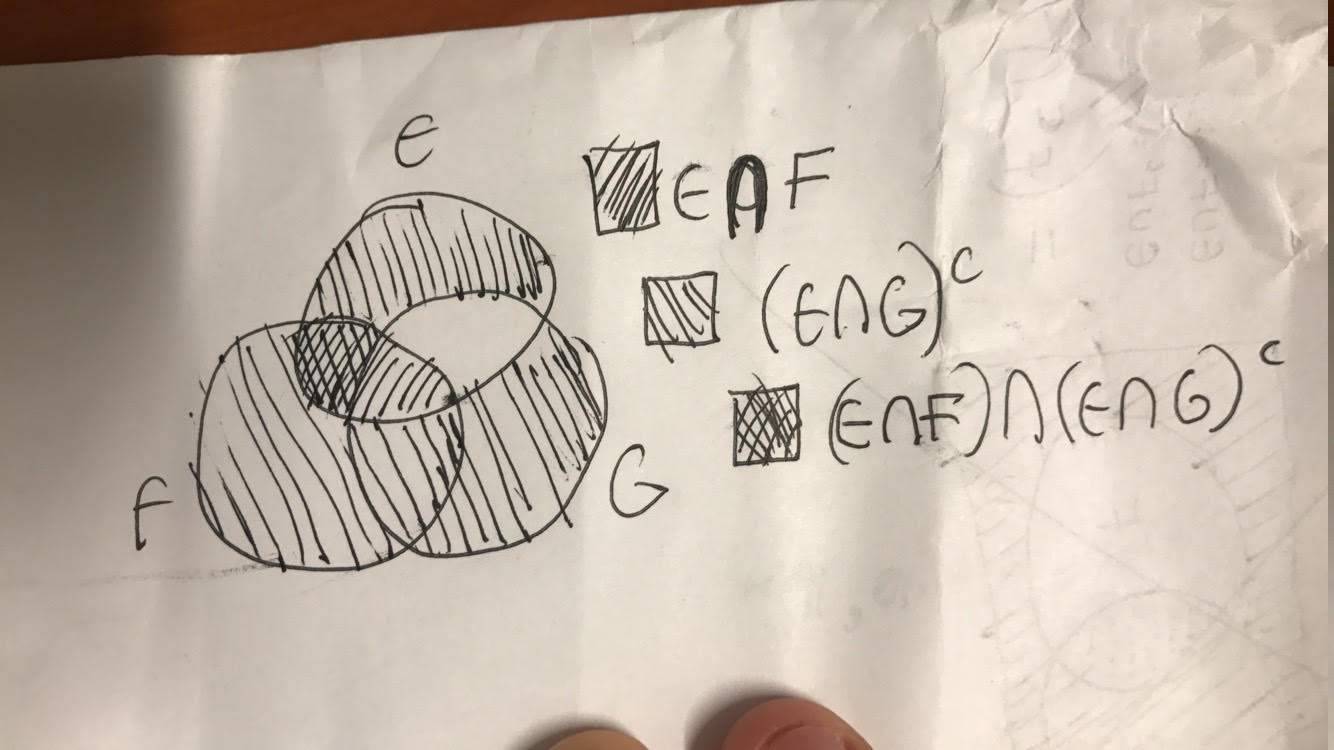
\includegraphics[width=400pt]{HW1P6b}
	\caption{Picture for Problem 6, part B. }
	\label{fig:hw1p6b}
\end{figure}

\noindent\rule{8cm}{0.4pt}

7. $P(A\cup B) = 0.76$, and $P(A\cup B') = 0.87$. 

For the first set, a simplification and placing in algebraic form gives:

$A + B = 0.76$

$A + B' = 0.87$

$B + B' = 1.00$

Placing in matrix form... 

$
\begin{bmatrix}
	1 & 1 & 0 \\
	1 & 0 & 1 \\
	0 & 1 & 1 \\
\end{bmatrix}
$

This is equal to 

$
\begin{bmatrix}
0.76  \\
0.87  \\
1.00  \\
\end{bmatrix}
$

Solving this system of matrices results in finding that $P(A) = 0.315$. 


\noindent\rule{8cm}{0.4pt}


8. There are $\boxed{12!}$ ways to line up the 12 children. If there are 6 boys and 6 girls, and the boys will all be in the back row, then there are $6!$ ways to arrange the boys, and $6!$ ways to arrange the girls. The order of the groups of children (not the order inside the groups) is already set, so there are $6! \times 6! = \boxed{518400}$ ways to arrange. 




























 

\end{document}